\documentclass[../report.tex]{subfiles}
\def\code#1{\texttt{#1}}
\begin{document}
\onehalfspacing

\pagebreak
\section{Verification}\label{sec:Verif}

In this section I will discuss the security properties used by each section of
Verified Boot. These properties have been mentioned earlier, but they are
formalized in this section.
Later in the section I verify these properties on the Hardware and
Software system that I outlined in Section 2 and Section 3.
Properties in software are checked using CBMC, where properties across the Hardware-Firmware boundary are checked using ILA.

All properties are being defined on the Read-Only Firmware of Verified boot.
The code for Verified Boot is taken from an unmodified vboot\_reference repository provided by Google. 
When secure promises cross the Hardware-Firmware boundary, they are evaluated
using the Hardware I selected in Section 2.
The Firmware that interacts with this Hardware was created by me, however it was 
modeled after the Firmware originally found in Google's Coreboot repository. 
If Google released the sources for their Hardware, then this testing could be
performed with no modification to the source code. 

%\subsection{Read-Only Fw Purpose}
%The Read-Only Firmware's purpose is to provide an initial configuration of the board's hardware and to verify the block of code that has been provided as the Read-Write Firmware.
%The RO Firmware requires the SHA and RSA accelerators to do cryptographic functions, and the TPM and Flash for secure storage.
%If Developer Mode or Recovery Mode are enabled then the Keyboard driver is required for user input and the Display driver is required for updating the user with the boot status.
%If Recovery Mode is enabled then the USB and SD drivers are required so that the recovery image can be read off of external storage.
%Implementations of all of these drivers are packaged with the RO Firmware so that the Vboot library can succeed.
%
%The first thing that RO Firmware is responsible for is loading in all of the Flash memory to RAM so that it is more easily accessible. 
%After Flash memory is in RAM, data structures like the GBB and the Firmware Image are populated by reading the flash map, which is always stored at a set location (see Figure~\ref{fig:fmap}).
%Once the data structures are populated and the hardware drivers are loaded, the RO Firmware moves into the Vboot library to verify the firmware image.
%
%% RO FW destinations
%The RO Vboot is responsible for checking the validity of the firmware image validity and either executing the code within the firmware image or failing appropriately.
%If the firmware image is insecure or the verification process fails for other reasons, it is likely that the system will be rebooted into recovery mode. 
%RO Vboot is responsible for setting a 32 bit flag known as a ``recovery reason'' for failure. This reason influences the Recovery process and is stored in the read write portion of Flash so that it is consistent across boots. 


\subsection{RO Firmware Properties}

The properties that we will be checking can be separated into 4 categories: array accesses, program flow, hyperproperties, and correctness.
The array access property restricts the writeable addresses in memory to valid array boundaries. 
Program flow properties refer to the execution path and function call stack throughout the program.
Correctness properties refer to facts about the code such that, if things were
designed successfully, certain states should not be reached.
Together these categories of properties should encompass each of claims that the system makes about security.

These properties will be specified in Computation Tree Logic (CTL). 
CTL adds temporal distinctions over propositional logic and this allows one to easily describe how a system changes over time.
The boolean connectives in propositional logic are $\lnot$ for NOT, $\land$ for
AND, $\lor$ for OR, and $p \to q$ for $p$ implies $q$.
CTL describes how propositional logic changes through time.
In CTL $Xp$ indicates that $p$ is true in the next state; $Fp$ indicates that $p$ is true eventually; $Gp$ indicates that $p$ is always true.

\subsubsection{Memory Access Locations}

Memory accesses in C are very important because the language allows for arbitrary addresses to be accessed. 
Addressing arrays before their starting address or after their final address is known as a buffer overrun and it is one of the most common security vulnerabilities. 
Buffer overruns allow a program to write or read to arbitrary memory. 
In this program, a buffer overrun could be used to modify the RSA public keys after they have been read in from secure storage, or it could modify the firmware image after it has been verified as secure. 
Such modifications would defeat the security purposes of Vboot and for this reason it is important to prevent the accessing of arrays past the array boundaries.
We can represent correct array accesses through formal specification using the formula below.

\begin{equation}
    G(a \to (i > 0 \land i < size(ptr)))
\end{equation}

In this equation $a$ is any array access, $ptr$ is the start of the array and $i$ is the access offset.
This equation states that for every memory access, the index is greater than 0 so it cannot access memory before the array,  and the index is smaller than the size of the array so memory after the array cannot be accessed.
Luckily, this problem is common enough that CBMC provides checking by default.
However, This equation on its own is not strong enough to provide array access security for verified boot. 
This is because Vboot uses pointer manipulation throughout in order to access structures and data within the Firmware Image. 
Verified boot reads the image in as one contiguous blob and then uses size and offset variables to read more information.
CBMC is not able to detect that this pointer manipulation is an out of bounds array access so this must be manually checked through the use of assertions each time something within the image is accessed.
The pointer manipulation can be expressed formally through the following formula.

\begin{equation}
    G(s \to \text{offset}(\text{struct}) + \text{size}(\text{struct}) <
    \text{size}(\text{img}) \land \text{offset}(\text{struct}) > 0)
\end{equation}

In this equation $s$ is each time a structure is created from a pointer dereference, $struct$ is the structure, and $img$ is the image that it is being pointed to.
The equation states that the offset and size of the struct do not go past the edge of the image and that the offset of the struct does is not negative or before the beginning of the image.

Together these properties state that array accesses must be in bounds and that structure dereferencing must be in bounds of the image that is being referenced.
As these are the two memory referencing techniques that have the potential for overrun, these properties protect the system against overrun attacks.

\subsubsection{Program Flow properties}

There needs to be an ordered constraint on the flow of the program. 
If the program flow is described formally then it will be easy to check that all stages of secure boot were called and in the correct order.
This will catch incorrect programs that skip steps and therefore skip verifying the image, or programs that execute steps out of order and therefore access data that has not been verified yet.
The graph for program flow is shown in Figure~\ref{fig:verif_flow}.
When verifying the flow of Vboot it is necessary to note that there are two firmware images stored in the system, Image A and Image B, and either can be used in the Vboot process. 
It is also necessary to note that Developer mode will skip a step in the verification process, and that this skipped step is a valid part of the Vboot flow.

Let $s_i$ correspond to the ith stage from Figure~\ref{fig:verif_flow} and $s_{ai}$ or $s_{bi}$ correspond to that stage for Image A or Image B respectively.

The equation below states that at any time, we must be in at least one of five stages for either image A or image B.
% Must be in a defined state
\begin{equation}
    G(\bigvee\limits_{i = 0}^{4} s_{ai} \lor s_{bi})
\end{equation}

The equation below states the transitions available for Image A.
Each i\textsuperscript{th} stage can transition either to itself or the following stage.
Image A also has the ability to fail and have a transition immediately to the first stage of verifying Image B.

% Image A transitions to next or to B
\begin{equation}
    G(s_{ai} \to s_{ai} \lor s_{ai+1} \lor s_{b0})
\end{equation}

Now we will describe the state transitions for Image B. 
They are similar to Image A but Image B is always tried secondarily and can only transition to the next stage. 
Image B cannot transition back to verifying Image A or there would be the possibilities of an infinite loop of verifying incorrect images.

% Image B transitions to next
\begin{equation}
    G(s_{bi} \to s_{bi} \lor s_{bi+1})
\end{equation}

The final equation refines the transition for state $s_0$ for Image A and B.
In Figure~\ref{fig:verif_flow} we can see that state $s_0$ can transition to either $s_1$ but it also has a special transition to $s_2$ that is only valid if Developer Mode is enabled.

% State 0 can skip state 1 if in Developer
\begin{equation}
    G(s_0 \to (s_0 \lor s_{1} \lor (M_D \land s_{2})))
\end{equation}

All together these equations fully describe the program flow graph in Figure~\ref{fig:verif_flow}. 
If these hold then steps will not be skipped in the verification process and we can be assured that verification of the image will be attempted in order.

% \subsubsection{Hyperproperties}

% TODO: Look at this later
% Verified boot contains many stages and each stage holds multiple flags and meta-data. 
% We want to make sure that untrusted information does not influence our booting sequence, be

\subsubsection{Correctness properties}

Correctness properties refer to the code itself and help to determine if it has been written correctly.
For Verified Boot, correctness properties are focusing on the correct attestation of the image and attempting to guarantee that an incorrect image cannot be marked as correct and loaded for execution.
For example, the following property states that if the system is not in developer mode and the signature verification fails, then the system will eventually reach the failure state for that image.
It is important that failure and passing is tracked on an image basis because it is possible for Image A to have a bad signature but for Vboot to verify and load a correct Image B.

% Signature is correct when not in Dev mode
\begin{equation} \label{eq:sig_cor}
 \lnot M_d \land \lnot \text{verifySignature(img, rootKey)} \to XF (\text{img.pass} = F)
\end{equation}

The following property states that if the hash of the image data does not match the hash stored in the image, then that specific image will eventually fail.

% Hash is correct always 
\begin{equation} \label{eq:hash_cor}
    \text{hash(img.data)} \neq \text{img.hash} \to XF (\text{img.pass} = F)
\end{equation}

The next property checks against the rollback attack. 
Rollback states that all image versions must be greater than or equal to the last seen image version that is kept in secure storage. 
This property claims that if the image version is lower than what is seen in secure storage, then the image will eventually fail.
Rollback is disabled on Recovery Mode and the property below reflects this fact.

% Version should be greater than previously seen when not in recovery
\begin{equation} \label{eq:rollback}
    \lnot M_r \land (\text{img.version} < \text{prevVersion}) \to XF (\text{img.pass} = F)
\end{equation}

The next property checks that if both images fail, then the Vboot process will fail and the system will eventually reboot into recovery mode.

% If both images fail then boot to recovery 
\begin{equation} \label{eq:both-fail}
    \lnot \text{imgA.pass} \land \lnot \text{imgB.pass} \to XF (\text{pass} = F)
\end{equation}

% TODO: maybe add a Dev wipe property

% TODO: maybe add a hardware return correctly property
% TODO: maybe add that if hash(image) = img.hash -> image = img

In the equations above, img refers to the image to be verified (either Image A or Image B)  and rootKey is Google's public key that has been loaded out of the gbb.
$M_d$ refers to developer mode being active and $M_r$ refers to recovery mode being active.
Img.version is the RW firmware version and prevVersion is the last seen version that is stored in the TPM\@.
These properties will be proved contrapositively, meaning that when verified boot passes we will check that the antecedent is also false.


\subsection{CBMC}

CBMC is a Bounded Model Checking program for the C language that is released by
Carnegie Mellon. 
A Bounded Model Checker is a tool that performs Formal Verification.
Model checking is a way to exhaustively prove whether a given model meets its
specification.
Model checking typically uses propositional logic or temporal logic. 
At its core, CBMC transforms a C program into binary logic and
then uses a SAT solver to check it against the user's specification. 
The specification is user defined, using an API of C functions defined by the
CBMC library. 

\begin{figure}
  \centering
  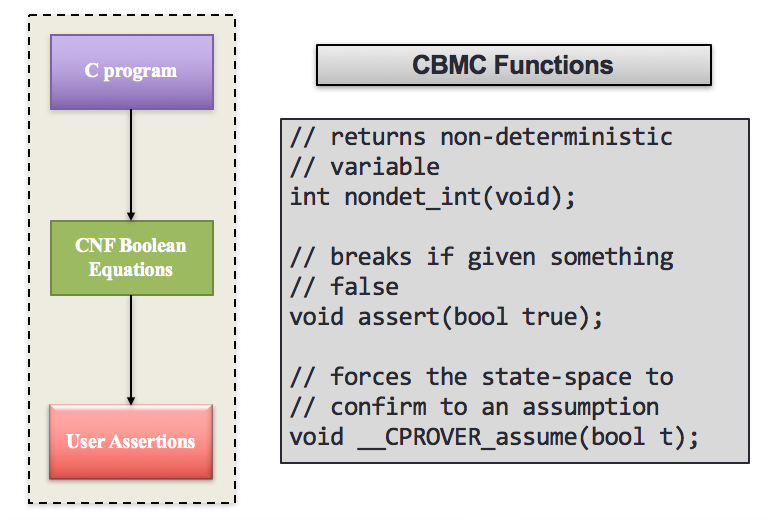
\includegraphics[width=0.8\linewidth]{CBMC_api.png}
  \caption{The figure on the left describes the transformation that a C
  program undergoes to be verified. The right describes the CBMC API.}\label{fig:CBMC_api}
\end{figure}

As we can see from Figure~\ref{fig:CBMC_api}, the CMBC API is very simple.
The \code{assert} function is the function used to describe the properties that
were outlined in the last section. 
The function takes in a boolean expression, and it is straightforward to
transform the propositional logic to a boolean expression in C.
If the boolean expression evaluates to \code{False}, then CBMC throws an error
and a ``counterexample''.
This counterexample is all of the program inputs and steps that led to this
assertion being False.
The \code{nondet\_int} function is used to model user input to the Vboot process.
Any data that could be modified by the user could feasibly take any
value.
To model this, \code{nondet\_int} is a function that returns a
``non-deterministic'' integer. 
Non-deterministic means the return integer can take any value, and CBMC
exhaustively checks user assertions against all possible integer values.

\subsubsection{Known CBMC Limitations}

In order to get CBMC running, certain limitations had to be observed.
The SAT generator of CBMC unrolls loops before converting the code into a model that can be checked.
This loop unroller is not able to unroll loops where the upperbound is data dependant, so these loops must either be avoided, or a limitation can be placed on the unrolling through the commandline. 
If the manually unrolling limitation is too small, then CBMC results may be incorrect, while if the limit is too large the state space may be too large for CMBC to finish in a reasonable time.
% TODO: may want to remove this bit about Memcpy
Luckily there was only a single loop of this nature, which existed in the method "Memcpy".
Using the C implementation of Vboot I was able to determine that Memcpy needed no more than 1050 loop unrollings for the data driven portion of Vboot.

\subsection{Verifying Vboot with CBMC}

CBMC was able to be successfully run on portions of the verified boot library and provide information on the satisfiability of various assertions.
Running CBMC on the Read-Only section of Vboot with a full Firmware Image is not possible as the program will consume up to 4GB of RAM on my local machine and then be cancelled.
In order to check properties, abstractions needed to be found such that parts of the Vboot flow could be checked at a single time.
The key insight that was used for this project is that individual functions are essentially self contained and can be abstracted away based on the properties that one desires to check.
Each function throughout Vboot returns an error code if it is not successful.
When a function is abstracted away, it is programmed to return a
non-deterministic value.
If the non-deterministic value is zero (success), then the minimal amount of external changes (if any) should be applied to the larger function.
If the abstracted function returns non-zero (error), then the external changes should be replaced with non-deterministic values.

This method is an over-abstraction of a functions found in the Vboot library.
An over-abstraction contains the full set of states found in the original function, plus additional states that would not be possible.
Because the over-abstraction is a super-set of the original states, any properties that are proved with the over-abstraction will also be proved on every state of the original function.
Therefore any properties proved with abstracted functions will also hold if the real functions were left in place.

\begin{figure}
  \centering
  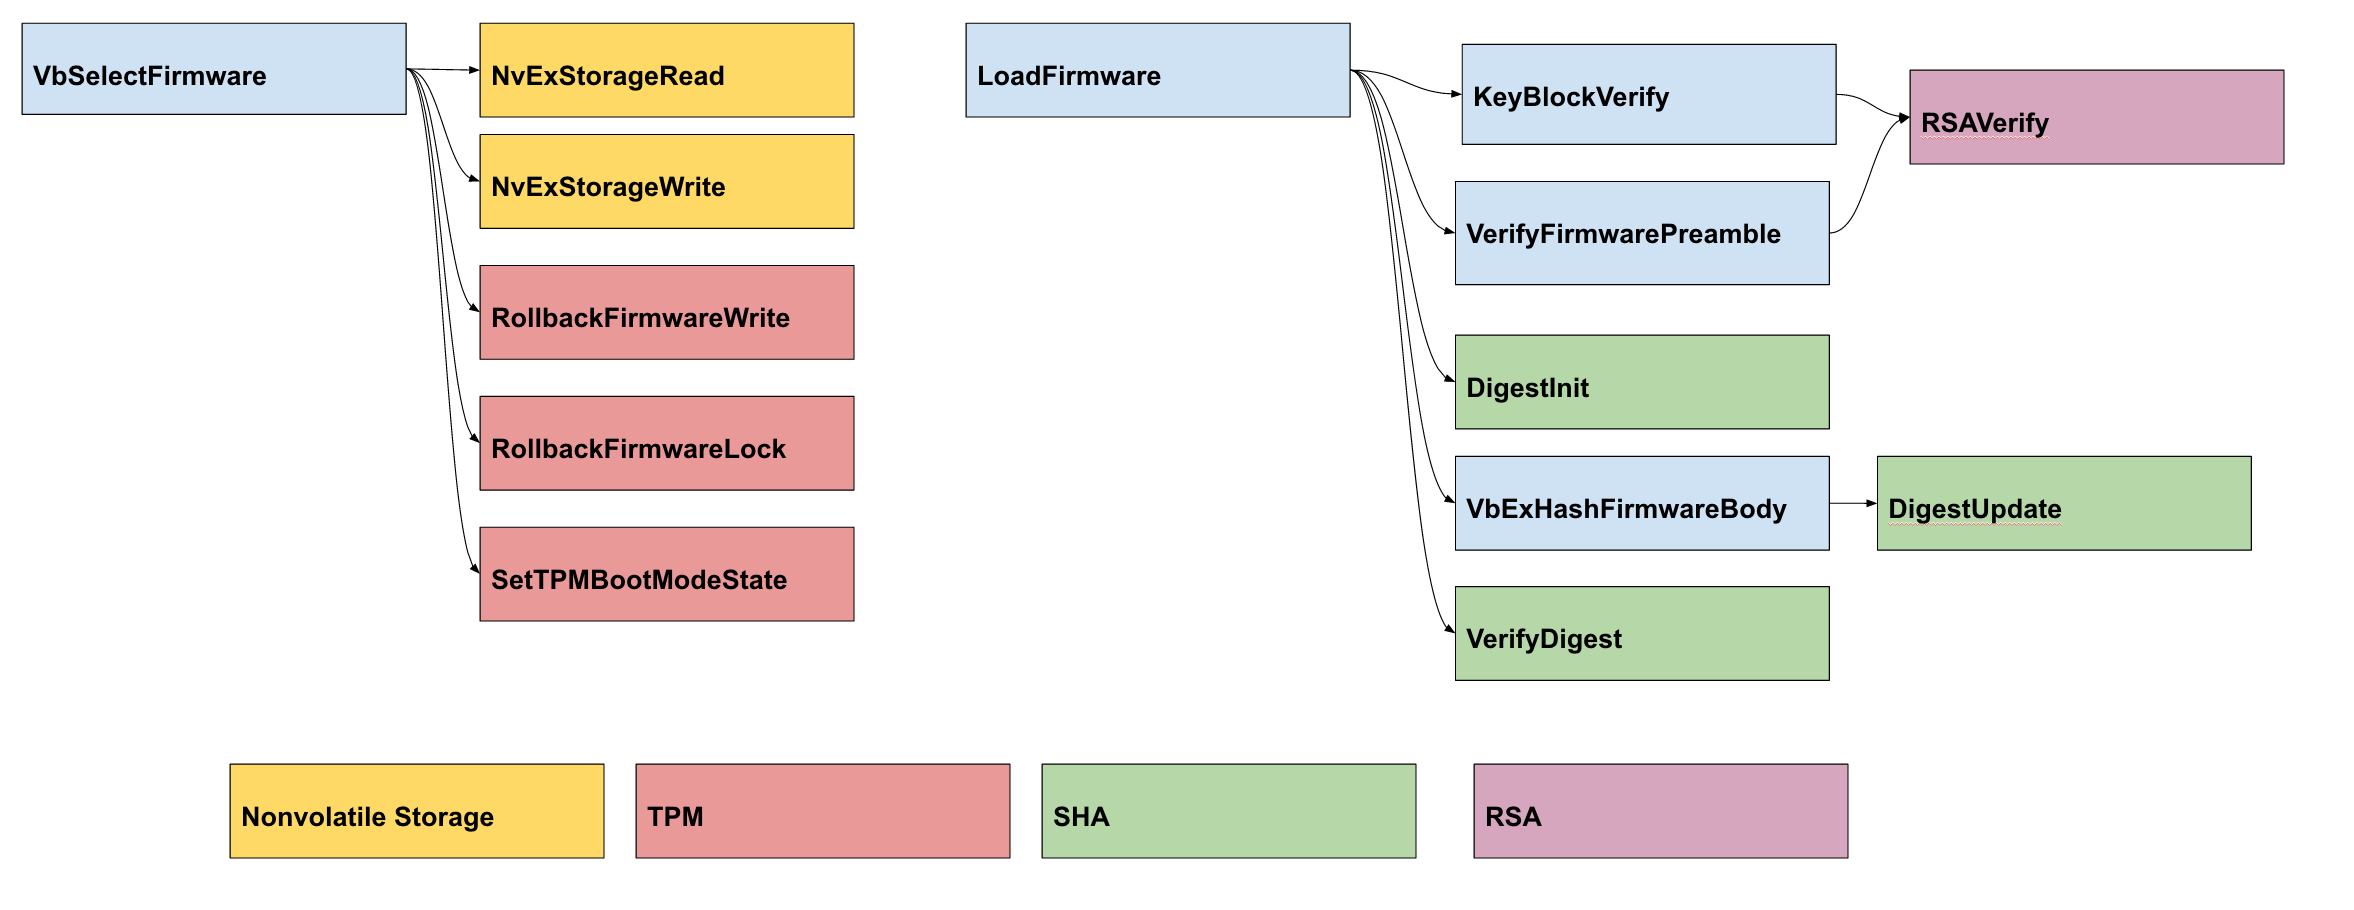
\includegraphics[width=0.8\linewidth]{ro_full_functions.png}
  \caption{The call graph of functions for Read Only Firmware}\label{fig:full_functions}
\end{figure}

The full graph of functions can be seen in Figure~\ref{fig:full_functions}.
The blue functions are fully software functions that are implemented in the Vboot Library.
The yellow functions connect to the Flash firmware on a real platform, but have been abstracted to return either non-deterministic data for Read-Write information, or hardcoded data for Read-Only information.
The red functions connect to the TPM on a real platform, but have been abstracted to return static variables are non-deterministic at the program's start.
The purple functions connect to either an RSA accelerator or a software RSA library. Instead of going through the full RSA algorithm, the function has been abstracted to a simple non-deterministic return of true or false. 
The green functions connect to either an SHA accelerator or a software SHA library.
The SHA algorithm has been abstracted in the same manner as RSA to return simply true or false at random.

For each of the next sections I will explain the verification process for individual functions. 
This explanation will include the function abstractions that were necessary, and a description of each of the tests run. 
There will be a table describing the results of each run of CBMC\@.
CMBC uses an implementation of a SAT solver known as the MiniSat solver\cite{minisat}.
This solver outputs unSAT if the assertions hold and SAT if they do not. 

\subsubsection{LoadFirmware}

The LoadFirmware function is where the main work is done in the Read-Only Vboot process.
LoadFirmware is responsible for calling functions that  Keyblock, Preamble, and Image verification.
When LoadFirmware returns, it will have set the pass or fail statuses of both Firmware Images.

All CBMC test results can be seen in Table~\ref{ldfw_results}. 
The Google unit tests involve adding a wrapper around Google's assertions within Vboot such that they hook into CBMC assertions.
This test shows that CMBC can be easily adapted into an existing framework and prove that Google specific assertions will not be thrown under any input.
The Rollback test checks that under no input conditions will LoadFirmware choose a firmware image with a lower version number (see Property~\ref{eq:rollback}).
In order to check that Rollback was working correctly, Rollback/rec tests that for rollback conditions without realizing that Rollback is allowed under recovery. 
The Rollback/Dev test correctly finds the counter-example where rollback is allowed and we can see that the recovery flag is enabled.
Hash Failure tests Property~\ref{eq:hash_cor}, or that it is impossible to verify an image as correct if the VbExHashFirmwareBody function returns an error.
RSA Failure tests Property~\ref{eq:sig_cor}, or that is impossible to verify an image as correct if the RSA key is formatted incorrectly or one of the Verify functions returns an error.
Array accesses check for all array bounds errors.

\begin{table}[]
    \centering
    \caption{CBMC tests on the LoadFirmware function}\label{ldfw_results}
    \begin{tabular}{|l|l|l|l|l|l|l|l|}
        \hline
        test name & steps & VCCs & vars  & clauses & time (s) & sat/unsat  \\ \hline \hline
        Google unit\_tests & 6460 & 34 & 1095643 & 24391723 & 67.02 & unsat \\ \hline
        rollback     & 4125 & 1 & 135239 & 1026823 & 4.79 & unsat \\ \hline
        rollback/rec & 4123 & 1 & 135276 & 1026983 & 4.68 & sat \\ \hline
        Hash Failure & 4182 & 2 & 137431 & 1043724 & 4.45 & unsat \\ \hline
        RSA  Failure & 4180 & 2 & 137825 & 1043921 & 4.45 & unsat \\ \hline
        Array Accesses & 4130 & 22 & 102660 & 640715 & 4.51 & unsat \\ \hline
    \end{tabular}
\end{table}

We can see from these tests that CBMC is working successfully and in a reasonable time.
The Google unit test framework is can be put to use with the CBMC framework using minor modifications, and the formal verification can be done in a very reasonable time.

\subsubsection{VbSelectFirmware}

The VbSelectFirmware function is the wrapper around LoadFirmware.
It is responsible for loading flags in from secure storage and for accessing the TPM\@.
VbSelectFirmware is also responsible for locking the TPM's firmware version before control passes to the firmware image and updating the version if a newer image has been loaded.
This function's final responsibility is to load TPM's PCR0 with the hash of the boot flags.

The TPM test for for this function is a series of correction properties. 
These assertions claim that the TPM must always be locked, and that VbSelectFirmware will not be successful if any of the TPM functions return an error.

The LoadFirmware test for this function simply checks that VbSelectFirmware will not not be successful if LoadFirmware returns an error.
This is necessary for the properties checked in LoadFirmware to propagate up to the entire boot flow, and it is what allows for our function abstractions.

\begin{table}[]
    \centering
    \caption{CBMC tests on function VbSelectFirmware}\label{sfw_results}
    \begin{tabular}{|l|l|l|l|l|l|l|l|}
        \hline
        test name & steps & VCCs & vars  & clauses & time (s) & sat/unsat  \\ \hline \hline
        TPM locking & 6 & 5269 & 13513 & 16784 & 0.07 & unsat \\ \hline
        LoadFirmware & 2 & 5264 & 13404 & 16209 & 0.07 & unsat \\ \hline
        Array Accesses & 5257 & 0 & 0 & 0 & 0 &  unsat \\ \hline
    \end{tabular}
\end{table}

\subsection{TPM Properties}

The Read-Only Firmware is responsible for setting up the TPM and protecting its
sections against the rest of the system that will eventually be loaded.
TPM's responsibilities from Chrome are to securely store the boot state and to protect against rollback attacks. 
Chrome's responsibilities for the TPM are to make sure that it is lead through
its self-check, that physical presence is disabled, and that the data zones
required by Chrome exist within the TPM's non-volatile state.

% Physical Presence
% http://www.trustedcomputinggroup.org/wp-content/uploads/Physical-Presence-Interface_1-30_0-52.pdf pg 19
Chrome disables the physical protection in the RO Firmware.
Physical presence is something that can be set high or low on a TPM either through software commands or a hardware wire. 
If Physical Presence is set high, then the ownership of the TPM can be changed and the re-provisioning operations become available.
For this reason, Chrome completely disables this option by permanently locking the TPM to a low Physical Presence\@.

% Rollback Attack
% TODO: Rollback attack visual
The other thing that the TPM protects from is Rollback Attacks.
In this situation a rollback attack is when older software with known
vulnerabilities replaces newer, protected software in a malicious ``upgrade.''
This attack works against a naive implementation because the attacker is relying on an older version of ChromeOS that is available, and unmodified.
Because the attacker is using Google's software, the software is signed by Google's private key and will be accepted by the VBoot algorithm.

\subsubsection{ILA for Hardware}   

\subsubsection{Verifying TPM with ILA}   
\clearpage

\end{document}
